\documentclass[12pt]{article}
\usepackage[a4paper, top=0.8in, bottom=0.7in, left=0.8in, right=0.8in]{geometry}
\usepackage{amsmath}
\usepackage{amsfonts}
\usepackage{amssymb} % For \checkmark
\usepackage{graphicx}
\usepackage{fancyhdr}
\usepackage{enumitem}
\usepackage{setspace}
\usepackage{tcolorbox}
\usepackage{xcolor}
\usepackage{tikz}
\usepackage[defaultfam,tabular,lining]{montserrat}
\usepackage[T1]{fontenc}
\renewcommand*\oldstylenums[1]{{\fontfamily{Montserrat-TOsF}\selectfont #1}}
\renewcommand{\familydefault}{\sfdefault}

\setlength{\headheight}{27.11148pt}

% Header Configuration
\pagestyle{fancy}
\fancyhf{}
\fancyhead[L]{Practice Exam D: Pre/Post-Test ANSWER KEY}
\fancyhead[R]{
\includegraphics[width=0.8cm]{Round Logo.png}}
\fancyfoot[C]{\footnotesize © Study Smart Tutors}

\begin{document}

\subsection*{Assessment D: Math Pre/Post-Test}
\onehalfspacing

\begin{tcolorbox}[colframe=black!50, colback=white, title=Assessment Directions]
\textbf{Directions:} Solve each question carefully. For multiple-choice questions, circle the best answer. For "select all that apply" questions, mark all correct answers. For short-answer questions, show your work clearly.
\end{tcolorbox}

% Problem 1: Multiplication Sentence (Write-In)
\begin{tcolorbox}[colframe=black!50, colback=white, title=\textbf{Problem 1}]
Write a multiplication sentence for the following situation: \\
``There are 4 baskets, and each basket has 6 apples.''  

\vspace{1cm}
\textbf{Answer:}  
\textcolor{red}{\[
4 \times 6 = 24 \text{ apples.}
\]}  
\textcolor{red}{\textbf{Explanation:} There are 4 groups (baskets), each containing 6 apples. Multiplying the two values gives the total number of apples: 24.}
\end{tcolorbox}

% Problem 2: Division Word Problem (Multiple Choice)
\begin{tcolorbox}[colframe=black!50, colback=white, title=\textbf{Problem 2}]
A classroom has 24 students. If the teacher wants to create groups of 6 students, how many groups will there be?  

\begin{enumerate}[label=(\Alph*)]
    \item 3
    \item 4
    \item 5
    \item 6
\end{enumerate}

\textcolor{red}{\[
\frac{24}{6} = 4
\]}  
\textcolor{red}{\textbf{Answer:} B) 4}  
\textcolor{red}{\textbf{Explanation:} Divide the total students (24) by the group size (6) to get 4 groups.}
\end{tcolorbox}

% Problem 3: Unknown Number in Equation (Write-In)
\begin{tcolorbox}[colframe=black!50, colback=white, title=\textbf{Problem 3}]
Find the missing number:  
\(8 \times \_\_\_ = 56\)  

\vspace{1cm}
\textbf{Answer:}  
\textcolor{red}{\[
8 \times 7 = 56
\]}  
\textcolor{red}{\textbf{Explanation:} Divide 56 by 8 to find the missing factor: \(56 \div 8 = 7\).}
\end{tcolorbox}

% Problem 4: Visual Multiplication (Performance Task)
\begin{tcolorbox}[colframe=black!50, colback=white, title=\textbf{Problem 4}]
Draw an array to represent \(3 \times 5\). Then write the multiplication equation to describe it.

\textbf{Answer:}  
\textcolor{red}{\textbf{Array:}}  

\begin{center}

\begin{tikzpicture}
    % Draw 3 rows and 5 columns of dots
    \foreach \x in {0,1,2,3,4} {
        \foreach \y in {0,1,2} {
            \filldraw (\x*0.7, -\y*0.7) circle (3pt);
        }
    }
\end{tikzpicture}
\end{center}

\textcolor{red}{\[
3 \times 5 = 15
\]}  
\textcolor{red}{\textbf{Explanation:} The array shows 3 rows with 5 dots in each row, representing \(3 \times 5\), which equals 15.}
\end{tcolorbox}

% Problem 5: Equivalent Equations (Select All That Apply with Boxes)
\begin{tcolorbox}[colframe=black!50, colback=white, title=\textbf{Problem 5}]
Select all the expressions that are equivalent to \(12\):  

\begin{itemize}[label=$\Box$]
    \item \textcolor{red}{\(4 \times 3 = 12\) \checkmark}
    \item \textcolor{red}{\(6 \times 2 = 12\) \checkmark}
    \item \textcolor{red}{\(12 \div 4 = 3\) \texttimes (incorrect, as this equals 3).}
    \item \textcolor{red}{\(5 + 2 = 12\) \texttimes (incorrect, as this equals 7).}
\end{itemize}
\end{tcolorbox}

% Problem 6: Division and Unknown Factor (Write-In)
\begin{tcolorbox}[colframe=black!50, colback=white, title=\textbf{Problem 6}]
Divide 45 cookies into 9 equal groups. How many cookies are in each group?  

\textbf{Answer:}  
\textcolor{red}{\[
\frac{45}{9} = 5 \text{ cookies per group.}
\]}  
\textcolor{red}{\textbf{Explanation:} Divide the total cookies (45) by the group count (9).}
\end{tcolorbox}

% Problem 7: Fractions on Number Line (Performance Task)
\begin{tcolorbox}[colframe=black!50, colback=white, title=\textbf{Problem 7}]
Mark \(1\frac{3}{4}\) on the number line below.

\textcolor{red}{\textbf{Solution:} Locate \(1.75\) on the number line. It is three-fourths of the way between 1 and 2.}
\end{tcolorbox}

% Problem 8: Two-Step Word Problem (Multiple Choice)
\begin{tcolorbox}[colframe=black!50, colback=white, title=\textbf{Problem 8}]
Maya reads 12 pages a day. How many pages will she read in 5 days if she reads the same number of pages each day?  

\begin{enumerate}[label=(\Alph*)]
    \item 50 pages
    \item 60 pages
    \item 72 pages
    \item 100 pages
\end{enumerate}

\textcolor{red}{\[
12 \times 5 = 60 \text{ pages.}
\]}  
\textcolor{red}{\textbf{Answer:} B) 60 pages.}
\end{tcolorbox}

% Problem 9: Shading Fractions (Performance Task)
\begin{tcolorbox}[colframe=black!50, colback=white, title=\textbf{Problem 9}]
Shade \(\frac{3}{4}\) of the diagram below.

\textbf{Answer:}  
\begin{center}
\begin{tikzpicture}
    % Draw 3x4 grid
    \foreach \x in {0,1,2,3} {
        \foreach \y in {0,1,2} {
            \draw[thick] (\x,\y) rectangle (\x+1,\y+1);
        }
    }
    % Shade 9 squares (3/4 of 12 squares)
    \foreach \x/\y in {0/0, 1/0, 2/0, 3/0, 0/1, 1/1, 2/1, 3/1, 0/2} {
        \fill[gray!50] (\x,\y) rectangle (\x+1,\y+1);
    }
\end{tikzpicture}
\end{center}

\textcolor{red}{\textbf{Solution:} Out of 12 total squares, shade 9 squares to represent \(\frac{3}{4}\).}
\end{tcolorbox}

% Problem 10: Estimation Word Problem (Write-In)
\begin{tcolorbox}[colframe=black!50, colback=white, title=\textbf{Problem 10}]
A store sells apples for \$3 each. John buys 12 apples. Estimate the total cost and explain your reasoning.

\textbf{Answer:}  
\textcolor{red}{\[
3 \times 12 = 36
\]}  
\textcolor{red}{\textbf{Explanation:} Multiply the price per apple (\$3) by the number of apples (12) to estimate the total cost as \$36.}
\end{tcolorbox}

\end{document}
